% This is LLNCS.DEM the demonstration file of
% the LaTeX macro package from Springer-Verlag
% for Lecture Notes in Computer Science,
% version 2.4 for LaTeX2e as of 16. April 2010
%
\documentclass{llncs}
%
\usepackage{makeidx}  % allows for indexgeneration
\usepackage{graphicx}
\usepackage{color}
\graphicspath{{figs/}} 	
\usepackage{array}	
\usepackage{multirow}
		
	
%
\begin{document}
%
\frontmatter          % for the preliminaries
%
\pagestyle{headings}  % switches on printing of running heads
\addtocmark{Hamiltonian Mechanics} % additional mark in the TOC
%

%
\mainmatter              % start of the contributions
%
\title{Discrimination of ADHD Based on fMRI Data with Deep Belief Network}
%
\titlerunning{Hamiltonian Mechanics}  % abbreviated title (for running head)
%                                     also used for the TOC unless
%                                     \toctitle is used
%
\author{Deping Kuang\inst{1} \and Xiaojiao Guo\inst{1}
 \and Xiu An\inst{1}  \and Yilu Zhao\inst{1} \and Lianghua He\inst{1}}
%
\authorrunning{Ivar Ekeland et al.} % abbreviated author list (for running head)
%
%%%% list of authors for the TOC (use if author list has to be modified)
\tocauthor{Ivar Ekeland, Roger Temam, Jeffrey Dean, David Grove,
Craig Chambers, Kim B. Bruce, and Elisa Bertino}
%
\institute{The Key Laboratory of Embedded System and Service Computing, Ministry of Education,
Tongji University, Shanghai 201804, China
,\\
Department of Computer Science and Technology, Tongji University, Shanghai 201804, China,\\
\email{kuangdp1990@gmail.com}}

\maketitle              % typeset the title of the contribution

\begin{abstract}
Effective discrimination of attention deficit hyperactivity disorder (ADHD) using imaging and functional biomarkers would have fundamental influence on public health. In this paper, we created a classification model using ADHD-200 dataset focusing on resting state functional magnetic resonance imaging (fMRI). We predicted ADHD status and subtype by deep belief network (DBN) and softmax, while DBN is used for feature extraction and softmax is applied to build a classifier to predict the subject as control, combined, inattentive or hyperactive. In the data preprocessing stage, in order to reduce the high dimension of fMRI brain data, brodmann mask, Fast Fourier Transform algorithm (FFT) and max-pooling of frequencies are applied respectively. Experimental results indicate that our method has a good discrimination effect, and outperform the results of the ADHD-200 competition. Meanwhile, our results conform to the biological research that there exists discrepancy in prefrontal cortex and cingulate cortex. As far as we know, it is the first time that the deep learning method has been used for the discrimination of ADHD with fMRI data.
\keywords{ADHD, fMRI, Deep Learning, Deep Belief Network}
\end{abstract}
%
\section{Introduction}
Attention deficit hyperactivity disorder (ADHD) is one of the most common childhood disorder and can continue through adolescence and adulthood with the problems of attention, hyperactivity, or acting impulsively\cite{1}. The American Psychiatric Association's Diagnostic and Statistical Manual, Fifth edition (DSM-5)\cite{2}, is usually used by mental health professionals to help diagnose ADHD. However, diagnose based on sole clinical and rating measure may be unreliable for it may have relationship with the clinicians, cultures and countries. Therefore, objective methods for diagnose of ADHD have great importance.


Functional magnetic resonance imaging (fMRI) is a functional neuroimaging technology, depending on blood oxygenation level dependent (BOLD), which defines activity in the healthy and diseased human brain\cite{3}. In recent years, a growing number of functional neuroimaging including task-related fMRI and resting-state fMRI have been applied in the research of ADHD. It is reported that abnormality of areas in the dorsal anterior cingulate cortex (dACC), ventro medial prefrontal cortex (vmPFC), and cerebellum when analysis task-related fMRI data\cite{4}\cite{5}. Wolf et al. [4] applied to 12 healthy and 12 ADHD adults using independent component analysis in a working memory task. Zhu et al\cite{6}. for the first time proposed a resting-state fMRI based PC-FDA classifier using features of regional homogeneity (ReHo) to discriminate children with ADHD from normal controls. The leave-one-out cross-validation accuracy can be as high as 85\%{}. But the subjects for the experiments were only 20. Due to the scarcity of data, few studies were for the automated diagnose of ADHD.Fortunately, the 1000 Functional Connectomes Project (FCP) provided a model which includes large-scale datasets\cite{7}. Upon this model, ADHD-200 Consortium established aggregate resting-state fMRI dataset and phenotypic data. On the global ADHD-200 competition, Eloyan A et al.\cite{8} from Johns Hopkins University achieved the best score but it is far from perfect. They mainly use rs-fc-fMRI based on decomposition of CUR along with gradient boosting. Furthermore, a motor network segmentation and random forest algorithm are used for prediction. In this paper, three datasets from ADHD-200 competition are applied to discriminate ADHD with typical controls. 


Deep belief network (DBN) is a generative probabilistic model which has raised a lot of interest since the successful implication of greedy layer-wise training using Restricted Boltzmann Machine (RBM)\cite{9}\cite{10}\cite{11}. DBN has been used to the application of image processing\cite{9}, audio classification\cite{12}, object recognition\cite{13}\cite{14}, natural language processing\cite{15} and so on. DBN models achieve good performance owing to the three distinct properties: it is a flexible neural network model; it has many non-linear hidden layers which makes it more flexible; it acts as a strong, domain-dependent regularization by generatively pertaining. However, DBN has never been applied to the discrimination of ADHD.


A deep belief network with three hidden layers is utilized to discriminate the ADHD of three types with control. Before using DBN, a series of process are conducted to correct the fMRI data from different backgrounds. To reduce the large dimension, brodmann mask, FFT and max-pooling of frequencies are performed. Deep belief network with softmax, which is for classification and fine-tuning the weights of network, is used for classifying the subject to the control or one subtype of ADHD. From the experimental results, it achieves higher accuracy than ever.


The sections below are our learning method and experiments. Section 2 mainly describes the RBM and DBN method and Section 3 presents our experimental results on ADHD dataset.


\section{Method}
The building blocks of a Deep Belief Network (DBN) are the Restricted Boltzmann Machines (RBMs), which are used to represent each layer of an DBN architecture.

%
\subsection{Restricted Boltzmann Machine}
%
A DBN is a hierarchical structure consisting of multiple stacked RBM. RBMs are undirected graphical models including two layers: visible units and hidden units (see Fig.\ref{fig:1}). The visible units that represent observations connect to the hidden units that represent features. But no connections are established within visible units or hidden units. The simplest RBM use Bernoulli distributed units in which the visible and hidden units are both binary. To adapt to the real-valued data, the Gaussian-Bernoulli RBMs with real-valued input for visible units and binary output for hidden units are used. It makes RBMs suitable to build blocks to learn DBNs for its valid greedy learning method.
\begin{figure}[!htbp]
	\centering 
		\includegraphics[scale=0.20]{figs/kdp1.jpeg}
    	\caption{Strcture of RBM} 
       	\label{fig:1}
\end{figure}


In RBMs, the joint probability distribution between $v$ and $h$ can be written as:
\begin{equation}
  P(v,h)=\frac{1}{Z}\exp(-E(v,h))
\end{equation}
Where $v$ is visible unit,$h$ is hidden unit, $E$ is an energy function defined by:
\begin{equation}
  E(v,h)=-\sum_{i=1}^{V}\sum_{j=1}^{H}v_ih_jw_{ij}-
  \sum_{i=1}^{V}b_iv_i-\sum_{j=1}^{H}a_jh_j
\end{equation}
$v_i,h_j \in {0,1}$,$w_{ij}$ is the weight between $v_i$ and $h_j$,$b_i$ is the bias of visible unit and $h_j$ is the bias of hidden unit.$Z$ is obtained by the sum computed by:
\begin{equation}
 Z=\sum_{v,h}e^{-E(v,h)}
\end{equation}
The probability of a visible unit which is assigned by the model is:
\begin{equation}
 p(v)=\frac{\sum_he^{-E(v,h)}}{\sum_v\sum_he^{-E(v,h)}}
\end{equation}
The conditional distributions $p(v|h)$ and $p(h|v)$ are given by:
\begin{equation}
 p(h_j=1|v;\theta)=\sigma(\sum_{i=1}^{V}w_{ij}v_j+a_j) 
\end{equation}
\begin{equation}
 p(h_i=1|h;\theta)=\sigma(\sum_{j=1}^{H}w_{ij}v_j+b_i)
\end{equation}
where $\theta=(w,b,a)$ and $\sigma(x)=(1+e^{-x})^-1$.


An RBM is pre-trained to maximize the log-likelihood $\log p(v)$. The derivative of the $\log$ probability with respect to the wights is given by:
\begin{equation}
\frac{\partial \log p(v)}{\partial \omega_{ij}}=\langle v_ih_j \rangle_v - 
\langle v_ih_j \rangle_{model}
\end{equation}
Where the angle brackets manifested the expectations relative to the distribution specified in the subscript. The update rule for the weights follows the gradient of the $\log$ likelihood as:
\begin{equation}
\Delta\omega_{ij}=\epsilon(\langle v_ih_j \rangle_{data} - 
\langle v_ih_j \rangle_{model})
\end{equation}
Where $\epsilon$ is the learning rate. It takes exponential time to compute the exact value of term $\langle v_ih_j \rangle_{model}$. But the Contrastive Divergence $\langle CD \rangle_{model}$ [16] approximation to the gradient can be used.Then the new update rule is:
\begin{equation}
\Delta\omega_{ij}=\epsilon(\langle v_ih_j \rangle_{data} - 
\langle v_ih_j \rangle_{recon})
\end{equation}
Where the term $\langle v_ih_j \rangle_{recon}$ represents the expectation of reconstructions produced by
initializing the data from the hidden units and then updating the hidden units according to the
data as visible units, it proves to work well in practice and to detect good features adequately.


\subsection{Deep Belief Networks}
After understanding how to build a RBM, it becomes much easier to construct a DBN by stacking RBMs. While the first RBM consisting of visible layer and first hidden layer is trained, the parameters,$\theta_1$, of this RBM is also obtained. It defines a prior distribution over first hidden units which is obtained by marginalizing over the space of visible units. The idea behind the DBN, which is training by a stack of RBMs, is to keep the $p(v|h,\theta_1)$ defined by the first RBM, but to improve $p(v)$ by replacing $p(h|\theta_1)$ by a better prior over the hidden units. The better prior must have a smaller Kullback-Leibler(KL) divergence than $p(h|\theta_1)$ from the aggregated posterior to improve $p(v)$. 


Considering training second RBM, which is the network formed by using samples from the aggregated posterior of first RBM as training data. It is simple to initialize the second RBM which has the visible and hidden units swapped in first RBM. Then the second RBM has visible units $h$ and hidden units $h_2$.We makes $p(h|\theta_2)$ be a better model of the aggregated posterior of $p(h|\theta_1)$ as the same of first RBM.


In the same way we could train a stack of RBMs. Then a feed-forward network of multiple layers can be initialized by the bottom-up recognition weights of the resulting DBN. The network can be fine-tuned by the back-propagating err derivatives, which is given by a final “softmax” layer that computes a probability over class labels. Softmax regression is also called multinomial logistic regression, which can deal with classification problem of the multi-class. In other words, it can be seen as the expansion of logistic regression. The weights in all lower layers are fine-tuned and the weights of final layer are back-propagated by the derivative of the log probability of the correct class. The process of bottom-up training and up-bottom fine-tuning is displayed in Fig.\ref{fig:2}.
\begin{figure}[!htbp]
	\begin{center}
		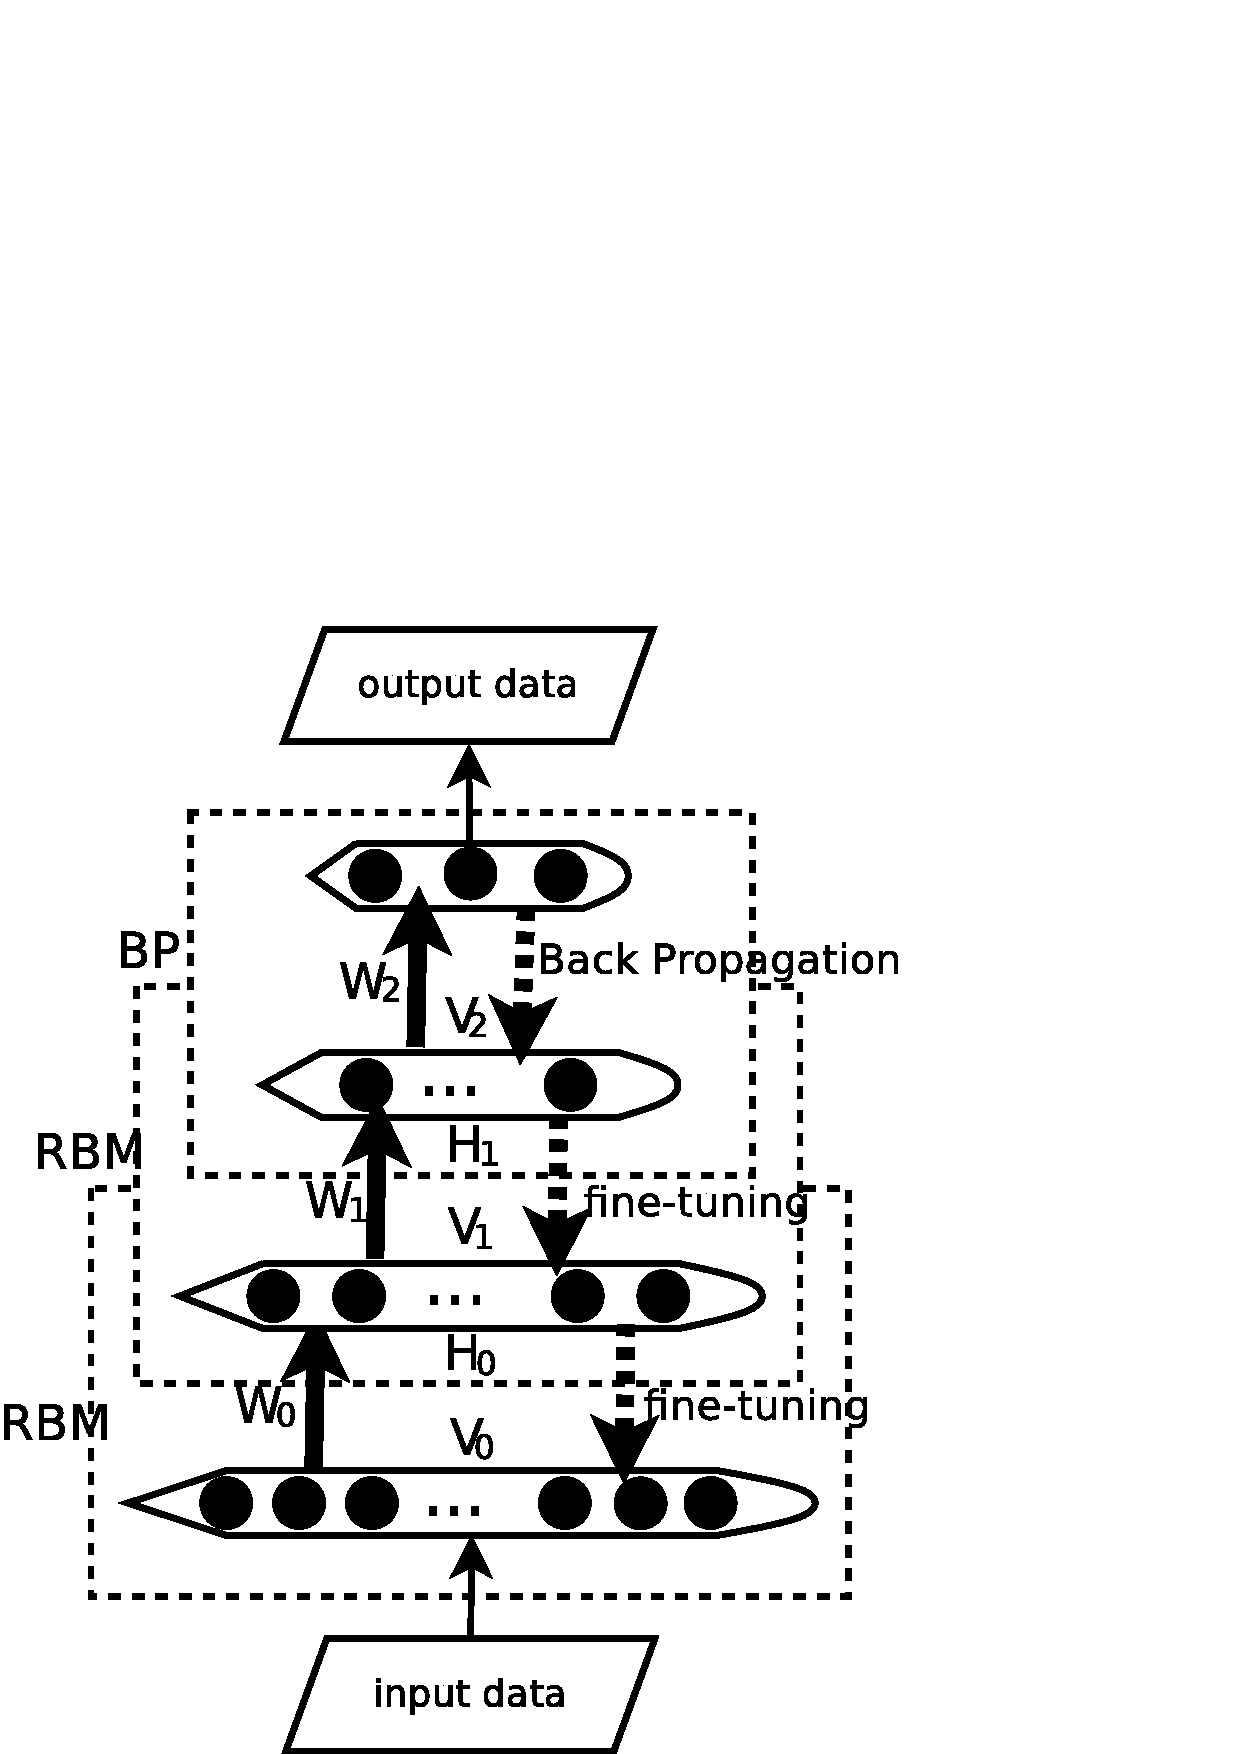
\includegraphics[scale=0.45]{figs/DBN.png}
	\end{center}
\caption{The process of DBN. The observation vectors are copied as the visible in the first RBM layer and the hidden vectors generated from the visible vectors in the first RBM are observed as the visible vectors in the second layer. Red arrows stands for the generative process and green arrows for the fine-tuning process. The top layer is a “softmax” which gives the class label of observations and back-propagate the weights between each layer in turn.}
\label{fig:2}
\end{figure}





\section{Experiments}
\subsection{Process of Data}
MRI data and scan parameters of ADHD were released on the ADHD-200 Global Competition website(\texttt{http://users/\homedir iekeland/web/welcome.html}). The fMRI data is time-series of 3D images which size is $49*58*47$. Due to the inevitable interference during the experimental procedure, in order to analysis data effectively, a series of preprocessing are conducted in spm8 [17] such as realign, slice time, co-register, normalize, smooth. More information about the preprocessing steps can be found in \cite{18}.


To reduce the dimension, three strategies are involved. First, divide the 3D images to 48 areas according to brodmann template which is a region of human cerebral cortex defined on its cytoaerchitectonics, or structure and organization of cells. Then, assume that the highest frequency of voxels in some areas may be different during the scanning procedure. So the fast Fourier transform algorithm (FFT) is used to transform data from time domain to frequency domain. At last, execute max-pooling of frequencies in each voxel to select the frequency which has the maximum value of amplitude. After FFT and max-pooling every voxels have only one property and the number of properties in each area depends on the number of voxels. We can use the properties for analysis after preprocessing.


\subsection{Application of DBN to ADHD data}
In this paper, we apply DBN to the preprocessed ADHD data for learning features of each area. The properties in each area are viewed as the observations of the first layer in the DBN, which is composed of three hidden layers training with greedy RBMs. The data collected by different institutions came from various experimental environment and scan parameters, so we discriminate the ADHD vs. Typically Developing Controls (TDC) separately by training different DBNs for different sites. The diagnose of each subject is given according to the DSM-5 with regard to the score of inattentive, hyper/impulsive, IQ measure and so on. Actually, for the data of every site we train 48 DBNs, and discriminate the class of subject by every DBN, for the numbers of observations are different from one area to another. Also, in order to exclude the occasionality of the data collected from individual area, we combined properties from some areas to one vector of features. The whole procedure is shown below in Fig.\ref{fig:3}.
\begin{figure}[!htbp]
	\centering
		\includegraphics[scale=0.30]{figs/procedure.jpg}
    	\caption{The procedure of DBN applied to ADHD data}
    	    	\label{fig:3} 
\end{figure}


\subsection{Results}
The ADHD-200 Global Competition divided the datasets into training and test sets. We test the DBN on the ADHD hold-out set for KKI, Peking-1 and NYU, with softmax as the classifier. For KKI dataset, the training subjects are 83, and test subjects are 11; for Peking-1 dataset, the training subjects are 85, and test subjects are 50; and for NYU the training subjects and test subjects are 222 and 41 respectively. The detailed information for the subjects is shown in Table \ref{tab:1}.

\begin{table}
\caption{Demographic information of KKI, Peking-1 and NYU}
\label{tab:1}
\begin{center}
\begin{tabular}{|c|c|c|c|c|c|c|}
\hline
\multirow{3}{*}{site}	& \multicolumn{2}{c|}{KKI} & \multicolumn{2}{c|}{Peking-1} & \multicolumn{2}{c|}{NYU} \\
\cline{2-7}\rule{0pt}{12pt}
					 	& training & \quad test \quad\quad & training	&\quad test\quad\quad	& taining & \quad test\quad\quad \\
						& 83		   & 11	  &    85   &   50  &   222   &   41 \\ [2pt]
\hline \rule{0pt}{12pt}
control					& 61		   & 8    &    61   &    27 &   99    &   12 \\
combined					& 16		   & 3    &    7    &    9  &   77    &   22 \\
inattentive				& 5		   & 0    &    0    &    1  &   44    &   0 \\
hyperactive				& 1		   & 0    &    17   &    13 &   2     &   7 \\[2pt]
\hline
\end{tabular}
\end{center}
\end{table}

As NYU dataset in the ADHD-200 competition achieved the lowest discrimination results. So in this paper, the proposed method was particularly tested on the NYU dataset of 48 areas to discriminate control with ADHD (regardless of subtypes). The results of 48 regions (excluding 7 empty regions) are shown in Fig.\ref{fig:4}. It can be inferred that the average discrimination performs effectively in the area of 9, 10 and 11, 18, 30. On the other hand, according to brodmann definition[20], area 9, 10, 11 stands for prefrontal cortex, area 18 plays a role in the visual cortex and area 30 is part of cingulate cortex, and the average accuracies of the visual cortex and cingulate cortex are more than 50\%. Thus we combine the data of prefrontal cortex (area 9, 10 and 11) to one vector of features, and carried the same operation for the data of visual cortex (area 17, 18 and 19) and the data of cingulate cortex (area 23, 24, 26, 29, 30, 31 and 32). Then use them as the input observations of the DBN. \\
\begin{figure}[!htbp]
	\begin{center}
		\includegraphics[scale=0.35]{figs/fig4.png}
	\end{center}    	
\caption{Discrimination accuracy of NYU in 48 areas. The horizontal axis stands for the number of area and the vertical axis stands for the average accuracy.}
\label{fig:4}  
\end{figure}





The average accuracy of the four classes, including control and three ADHD subtypes, is shown in Table 2. It can be seen that the accuracy of the method we proposed above is better than the discrimination accuracy achieved by the team in the ADHD-200 competition which are 35.19\%, 51.05\% and 61.90\% for NYU, Peking-1 and KKI respectively. By performing DBN on prefrontal cortex, our average accuracies are 37.41\%, 54.00\% and 71.82\%. Compared with the competition results, our accuracy respectively improved 2.22 percent, 2.95 percent and 9.92 percent, which is shown in Table \ref{tab:4}. Meanwhile, the accuracies on cingulate cortex are 37.07\%, 54.00\% and 72.73\%, which is also higher than the accuracies of ADHD-200 compitition. However, the accuracies are lower on visual cortex since the subjects were scanning on the resting state. The results are receivable as it has been confirmed that there indeed exists disparity in prefrontal cortex and cingulate cortex between control and ADHD[21].The details are shown in Table  \ref{tab:3} and Table \ref{tab:4} showing the discrimination accuracy and performance improvement respectively. All the results above demonstrate that our method can obtain a better performance.



\begin{table}
\caption{Classification accuracy}
\label{tab:3}
\begin{center}
\begin{tabular}{ccccc}
\hline	\rule{0pt}{12pt}
site	&	ADHD-200 \qquad & prefrontal cortex \qquad&	visual cortex \qquad& cingulate cortex  \\[2pt]
\hline	\rule{0pt}{12pt}
NYU		&	35.19	&	37.41	&	34.39  & 37.07 \\
PEKING-1&	51.05	&	54.00	& 	51.20	&	54.00\\
KKI		&	61.90	&	71.82	&	68.82	& 72.73\\[2pt]
\hline
\end{tabular}
\end{center}
\end{table}


\begin{table}
\caption{Classification accuracy}
\label{tab:4}
\begin{center}
\begin{tabular}{ccccc}
\hline	\rule{0pt}{12pt}
site	&	ADHD-200 \qquad & prefrontal cortex \qquad&	visual cortex \qquad& cingulate cortex  \\[2pt]
\hline	\rule{0pt}{12pt}
NYU		&	35.19	&	37.41	&	34.39  & 37.07 \\
PEKING-1&	51.05	&	54.00	& 	51.20	&	54.00\\
KKI		&	61.90	&	71.82	&	68.82	& 72.73\\[2pt]
\hline
\end{tabular}
\end{center}
\end{table}


\section{Conclusion}
In this paper, deep belief network, one of the deep learning models, is applied for feature extraction. Experiments were carried out on NYU, Peking-1 and KKI. The proposed method was proved to be effective in discriminating between ADHD and control. And the accuracy of classification has improved in some degree compared with the results published in ADHD-200 competition. It may be feasible to apply this method to other studies on psychiatric disorders.


This results use part of brain regions but achieves better performance, and verifies that there is difference between ADHD and control in prefrontal cortex and cingulate cortex. In the future, we will expand our research brain regions, which may leads to a better discrimination performance. What's more, it is worth considering to take the personal characteristic data as well as fMRI-based information into analysis as described in [22]. By considering the above factors, there is a reason to believe that the discrimination performance based on the proposed method can be more effective.  



%
% ---- Bibliography ----
%
\begin{thebibliography}{}
%
\bibitem{1}
Kooij, S. J., Bejerot, S., Blackwell, A., Caci, H., Casas-Brugué, M., Carpentier, P. J., \& Asherson, P.: European consensus statement on diagnosis and treatment of adult ADHD: The European Network Adult ADHD. BMC psychiatry. 10(1), 67 (2010)
\bibitem{2}
American Psychiatric Association: The Diagnostic and Statistical Manual of Mental Disorders: DSM 5. bookpointUS. (2013)
\bibitem{3}
Huettel, S. A., Song, A. W., \& McCarthy, G.: Functional magnetic resonance imaging (Vol. 1). Sunderland, MA: Sinauer Associates. (2004)
\bibitem{4}
Wolf, R. C., Plichta, M. M., Sambataro, F., Fallgatter, A. J., Jacob, C., Lesch, K. P., \& Vasic, N.: Regional brain activation changes and abnormal functional connectivity of the ventrolateral prefrontal cortex during working memory processing in adults with attention‐deficit/hyperactivity disorder. Human brain mapping. 30(7), 2252-2266 (2009)
\bibitem{5}
Rubia, K., Cubillo, A., Smith, A. B., Woolley, J., Heyman, I., \& Brammer, M. J.: Disorder‐specific dysfunction in right inferior prefrontal cortex during two inhibition tasks in boys with attention‐deficit hyperactivity disorder compared to boys with obsessive–compulsive disorder. Human brain mapping. 31(2), 287-299 (2010) 
\bibitem{6}
Zhu, C. Z., Zang, Y. F., Cao, Q. J., Yan, C. G., He, Y., Jiang, T. Z., \& Wang, Y. F.: Fisher discriminative analysis of resting-state brain function for attention-deficit/hyperactivity disorder. Neuroimage. 40(1), 110-120 (2008)
\bibitem{7}
Milham, M. P.: Open neuroscience solutions for the connectome-wide association era. Neuron. 73(2), 214-218 (2012) 
\bibitem{8}
Eloyan, A., Muschelli, J., Nebel, M. B., Liu, H., Han, F., Zhao, T., \& Caffo, B.: Automated diagnoses of attention deficit hyperactive disorder using magnetic resonance imaging. (2012)
\bibitem{9}
Hinton, G. E., \& Salakhutdinov, R. R.: Reducing the dimensionality of data with neural networks. Science. 313(5786), 504-507 (2006)
\bibitem{10}
Hinton, G. E., Osindero, S., \& Teh, Y. W.: A fast learning algorithm for deep belief nets. Neural computation. 18(7), 1527-1554 (2006)
\bibitem{11}
Bengio, Y., Lamblin, P., Popovici, D., \& Larochelle, H.: Greedy layer-wise training of deep networks. Advances in neural information processing systems. 19, 153 (2007)
\bibitem{12}
Lee, H., Pham, P. T., Largman, Y., \& Ng, A. Y.: Unsupervised feature learning for audio classification using convolutional deep belief networks. NIPS. 9,1096-1104 (2009)

\bibitem{13}
Lee, H., Grosse, R., Ranganath, R., \& Ng, A. Y.: Unsupervised learning of hierarchical representations with convolutional deep belief networks. Communications of the ACM. 54(10), 95-103 (2011) 
\bibitem{14}
Ranzato, M., Huang, F. J., Boureau, Y. L., \& Lecun, Y.: Unsupervised learning of invariant feature hierarchies with applications to object recognition. In Computer Vision and Pattern Recognition. IEEE Conference on. IEEE 1-8 (2007)
\bibitem{15}
Sarikaya, R., Hinton, G. E., \& Deoras, A: Application of Deep Belief Networks for Natural Language Understanding. 
\bibitem{16}
Hinton, G. E.: Training products of experts by minimizing contrastive divergence. Neural computation. 14(8), 1771-1800 (2002)
\bibitem{17}
Friston, K. J.: Statistical parametric mapping. In Neuroscience Databases. Springer US. 237-250 (2003)
\bibitem{18}
Matthews, P. M., \& Jezzard, P.: Functional magnetic resonance imaging. Journal of Neurology, Neurosurgery \& Psychiatry. 75(1), 6-12 (2004)
\bibitem{19}
Bush, G., Frazier, J. A., Rauch, S. L., Seidman, L. J., Whalen, P. J., Jenike, M. A., \& Biederman, J.: Anterior cingulate cortex dysfunction in attention-deficit/hyperactivity disorder revealed by fMRI and the Counting Stroop. Biological psychiatry. 45(12), 1542-1552 (1999)
\bibitem{20} 
Wanchai: Cortical Functions. Trans Cranial Technologies ldt. (2012)
\bibitem{21}
Bush, G., Valera, E. M., \& Seidman, L. J.: Functional neuroimaging of attention-deficit/hyperactivity disorder: a review and suggested future directions. Biological psychiatry. 57(11), 1273-1284 (2005) 
\bibitem{22}
ADHD-200 Consortium.: The ADHD-200 consortium: a model to advance the translational potential of neuroimaging in clinical neuroscience.Frontiers in systems neuroscience. 6 (2012)

\end{thebibliography}

\end{document}
